\chapter{Fluxos e cortes}

Neste capítulo, vamos nos concentrar nos seguintes
dois problemas:

\begin{itemize}
\item \key{Encontrar um fluxo máximo}:
Qual é a quantidade máxima de fluxo que podemos
enviar de um nó para outro nó?
\item \key{Encontrar um corte mínimo}:
Qual é o conjunto de arestas de peso mínimo
que separa dois nós do grafo?
\end{itemize}

A entrada para ambos os problemas é um grafo direcionado e
ponderado que contém dois nós especiais:
a \emph{fonte} é um nó sem arestas de entrada,
e o \emph{sumidouro} é um nó sem arestas de saída.

Como exemplo, usaremos o seguinte grafo
onde o nó 1 é a fonte e o nó 6
é o sumidouro:

\begin{center}
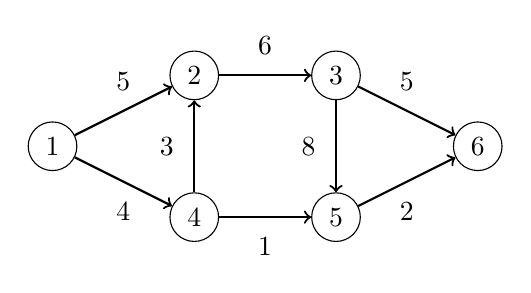
\begin{tikzpicture}[scale=0.9]
\node[draw, circle] (1) at (1,2) {$1$};
\node[draw, circle] (2) at (3,3) {$2$};
\node[draw, circle] (3) at (5,3) {$3$};
\node[draw, circle] (4) at (7,2) {$6$};
\node[draw, circle] (5) at (3,1) {$4$};
\node[draw, circle] (6) at (5,1) {$5$};
\path[draw,thick,->] (1) -- node[font=\small,label=5] {} (2);
\path[draw,thick,->] (2) -- node[font=\small,label=6] {} (3);
\path[draw,thick,->] (3) -- node[font=\small,label=5] {} (4);
\path[draw,thick,->] (1) -- node[font=\small,label=below:4] {} (5);
\path[draw,thick,->] (5) -- node[font=\small,label=below:1] {} (6);
\path[draw,thick,->] (6) -- node[font=\small,label=below:2] {} (4);
\path[draw,thick,<-] (2) -- node[font=\small,label=left:3] {} (5);
\path[draw,thick,->] (3) -- node[font=\small,label=left:8] {} (6);
\end{tikzpicture}
\end{center}

\subsubsection{Fluxo máximo}

\index{fluxo}
\index{fluxo máximo}

No problema do \key{fluxo máximo},
nossa tarefa é enviar o máximo de fluxo possível
da fonte para o sumidouro.
O peso de cada aresta é uma capacidade que
restringe o fluxo
que pode passar pela aresta.
Em cada nó intermediário,
o fluxo de entrada e o de saída
devem ser iguais.

Por exemplo, o tamanho máximo de um fluxo
no grafo de exemplo é 7.
A figura a seguir mostra como podemos
rotear o fluxo:

\begin{center}
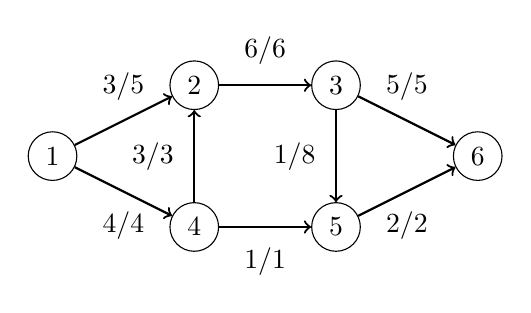
\begin{tikzpicture}[scale=0.9]
\node[draw, circle] (1) at (1,2) {$1$};
\node[draw, circle] (2) at (3,3) {$2$};
\node[draw, circle] (3) at (5,3) {$3$};
\node[draw, circle] (4) at (7,2) {$6$};
\node[draw, circle] (5) at (3,1) {$4$};
\node[draw, circle] (6) at (5,1) {$5$};
\path[draw,thick,->] (1) -- node[font=\small,label=3/5] {} (2);
\path[draw,thick,->] (2) -- node[font=\small,label=6/6] {} (3);
\path[draw,thick,->] (3) -- node[font=\small,label=5/5] {} (4);
\path[draw,thick,->] (1) -- node[font=\small,label=below:4/4] {} (5);
\path[draw,thick,->] (5) -- node[font=\small,label=below:1/1] {} (6);
\path[draw,thick,->] (6) -- node[font=\small,label=below:2/2] {} (4);
\path[draw,thick,<-] (2) -- node[font=\small,label=left:3/3] {} (5);
\path[draw,thick,->] (3) -- node[font=\small,label=left:1/8] {} (6);
\end{tikzpicture}
\end{center}

A notação $v/k$ significa
que um fluxo de $v$ unidades está sendo roteado através de
uma aresta cuja capacidade é de $k$ unidades.
O tamanho do fluxo é $7$,
pois a fonte envia $3+4$ unidades de fluxo
e o sumidouro recebe $5+2$ unidades de fluxo.
É fácil ver que este fluxo é máximo,
pois a capacidade total das arestas
que levam ao sumidouro é $7$.

\subsubsection{Corte mínimo}

\index{corte}
\index{corte mínimo}

No problema do \key{corte mínimo},
nossa tarefa é remover um conjunto
de arestas do grafo
de forma que não haja caminho da fonte
ao destino após a remoção
e o peso total das arestas removidas
seja mínimo.

O tamanho mínimo de um corte no grafo de exemplo é 7.
Basta remover as arestas $2 \rightarrow 3$
e $4 \rightarrow 5$:

\begin{center}
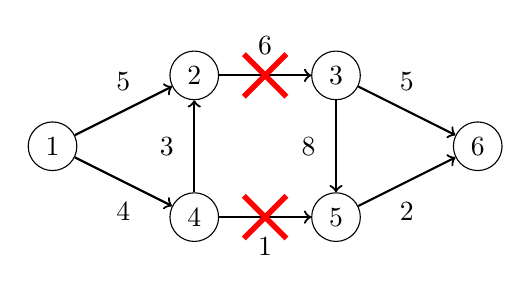
\begin{tikzpicture}[scale=0.9]
\node[draw, circle] (1) at (1,2) {$1$};
\node[draw, circle] (2) at (3,3) {$2$};
\node[draw, circle] (3) at (5,3) {$3$};
\node[draw, circle] (4) at (7,2) {$6$};
\node[draw, circle] (5) at (3,1) {$4$};
\node[draw, circle] (6) at (5,1) {$5$};
\path[draw,thick,->] (1) -- node[font=\small,label=5] {} (2);
\path[draw,thick,->] (2) -- node[font=\small,label=6] {} (3);
\path[draw,thick,->] (3) -- node[font=\small,label=5] {} (4);
\path[draw,thick,->] (1) -- node[font=\small,label=below:4] {} (5);
\path[draw,thick,->] (5) -- node[font=\small,label=below:1] {} (6);
\path[draw,thick,->] (6) -- node[font=\small,label=below:2] {} (4);
\path[draw,thick,<-] (2) -- node[font=\small,label=left:3] {} (5);
\path[draw,thick,->] (3) -- node[font=\small,label=left:8] {} (6);

\path[draw=red,thick,-,line width=2pt] (4-.3,3-.3) -- (4+.3,3+.3);
\path[draw=red,thick,-,line width=2pt] (4-.3,3+.3) -- (4+.3,3-.3);
\path[draw=red,thick,-,line width=2pt] (4-.3,1-.3) -- (4+.3,1+.3);
\path[draw=red,thick,-,line width=2pt] (4-.3,1+.3) -- (4+.3,1-.3);
\end{tikzpicture}
\end{center}

Após a remoção das arestas,
não haverá caminho da fonte para o sumidouro.
O tamanho do corte é $7$,
pois os pesos das arestas removidas
são $6$ e $1$.
O corte é mínimo, pois não há maneira válida
de remover arestas do grafo de forma que
seu peso total seja menor que $7$.
\\\\
Não é uma coincidência que
o tamanho máximo de um fluxo
e o tamanho mínimo de um corte
sejam iguais no exemplo acima.
Acontece que um fluxo máximo
e um corte mínimo são
\emph{sempre} igualmente grandes,
então os conceitos são dois lados da mesma moeda.

Em seguida, discutiremos o algoritmo de Ford–Fulkerson
que pode ser usado para encontrar
o fluxo máximo e o corte mínimo de um grafo.
O algoritmo também nos ajuda a entender
\emph{por que} eles são igualmente grandes.

\section{Algoritmo de Ford–Fulkerson}

\index{Algoritmo de Ford–Fulkerson}

O \key{algoritmo de Ford–Fulkerson} \cite{for56} encontra
o fluxo máximo em um grafo.
O algoritmo começa com um fluxo vazio,
e a cada passo encontra um caminho da fonte
para o sumidouro que gera mais fluxo.
Finalmente, quando o algoritmo não consegue mais aumentar o fluxo,
o fluxo máximo foi encontrado.

O algoritmo utiliza uma representação especial
do grafo em que cada aresta original possui uma aresta reversa
em outra direção.
O peso de cada aresta indica quanto mais fluxo
poderia ser direcionado por ela.
No início do algoritmo, o peso de cada aresta original
é igual à capacidade da aresta
e o peso de cada aresta reversa é zero.

\begin{samepage}
A nova representação para o grafo de exemplo é a seguinte:

\begin{center}
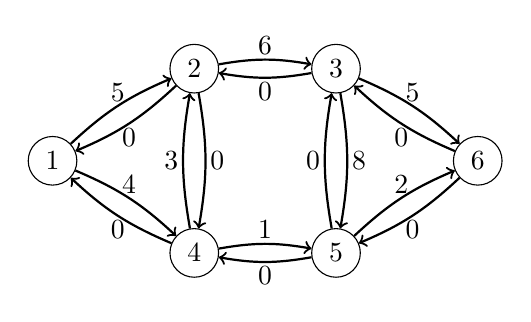
\begin{tikzpicture}[scale=0.9,label distance=-2mm]
\node[draw, circle] (1) at (1,1.3) {$1$};
\node[draw, circle] (2) at (3,2.6) {$2$};
\node[draw, circle] (3) at (5,2.6) {$3$};
\node[draw, circle] (4) at (7,1.3) {$6$};
\node[draw, circle] (5) at (3,0) {$4$};
\node[draw, circle] (6) at (5,0) {$5$};

\path[draw,thick,->] (1) edge [bend left=10] node[font=\small,label=5] {} (2);
\path[draw,thick,->] (2) edge [bend left=10] node[font=\small,label=below:0] {} (1);
\path[draw,thick,->] (2) edge [bend left=10] node[font=\small,label=6] {} (3);
\path[draw,thick,->] (3) edge [bend left=10] node[font=\small,label=below:0] {} (2);
\path[draw,thick,->] (3) edge [bend left=10] node[font=\small,label=5] {} (4);
\path[draw,thick,->] (4) edge [bend left=10] node[font=\small,label=below:0] {} (3);
\path[draw,thick,->] (1) edge [bend left=10] node[font=\small,label=4] {} (5);
\path[draw,thick,->] (5) edge [bend left=10] node[font=\small,label=below:0] {} (1);
\path[draw,thick,->] (5) edge [bend left=10] node[font=\small,label=1] {} (6);
\path[draw,thick,->] (6) edge [bend left=10] node[font=\small,label=below:0] {} (5);
\path[draw,thick,->] (6) edge [bend left=10] node[font=\small,label=2] {} (4);
\path[draw,thick,->] (4) edge [bend left=10] node[font=\small,label=below:0] {} (6);
\path[draw,thick,->] (5) edge [bend left=10] node[font=\small,label=left:3] {} (2);
\path[draw,thick,->] (2) edge [bend left=10] node[font=\small,label=right:0] {} (5);
\path[draw,thick,->] (3) edge [bend left=10] node[font=\small,label=right:8] {} (6);
\path[draw,thick,->] (6) edge [bend left=10] node[font=\small,label=left:0] {} (3);
\end{tikzpicture}
\end{center}
\end{samepage}

\subsubsection{Descrição do algoritmo}

O algoritmo de Ford–Fulkerson consiste em várias
rodadas.
Em cada rodada, o algoritmo encontra
um caminho da fonte para o sumidouro
tal que cada aresta no caminho tenha um peso positivo.
Se houver mais de um caminho possível disponível,
podemos escolher qualquer um deles.

Por exemplo, suponha que escolhemos o seguinte caminho:

\begin{center}
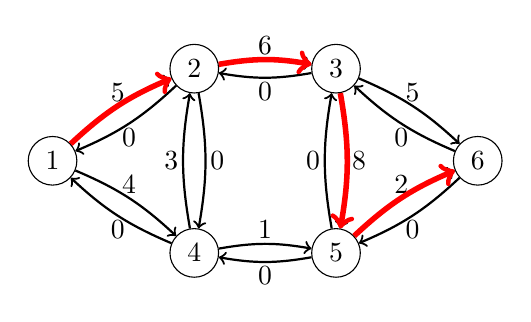
\begin{tikzpicture}[scale=0.9,label distance=-2mm]
\node[draw, circle] (1) at (1,1.3) {$1$};
\node[draw, circle] (2) at (3,2.6) {$2$};
\node[draw, circle] (3) at (5,2.6) {$3$};
\node[draw, circle] (4) at (7,1.3) {$6$};
\node[draw, circle] (5) at (3,0) {$4$};
\node[draw, circle] (6) at (5,0) {$5$};

\path[draw,thick,->] (1) edge [bend left=10] node[font=\small,label=5] {} (2);
\path[draw,thick,->] (2) edge [bend left=10] node[font=\small,label=below:0] {} (1);
\path[draw,thick,->] (2) edge [bend left=10] node[font=\small,label=6] {} (3);
\path[draw,thick,->] (3) edge [bend left=10] node[font=\small,label=below:0] {} (2);
\path[draw,thick,->] (3) edge [bend left=10] node[font=\small,label=5] {} (4);
\path[draw,thick,->] (4) edge [bend left=10] node[font=\small,label=below:0] {} (3);
\path[draw,thick,->] (1) edge [bend left=10] node[font=\small,label=4] {} (5);
\path[draw,thick,->] (5) edge [bend left=10] node[font=\small,label=below:0] {} (1);
\path[draw,thick,->] (5) edge [bend left=10] node[font=\small,label=1] {} (6);
\path[draw,thick,->] (6) edge [bend left=10] node[font=\small,label=below:0] {} (5);
\path[draw,thick,->] (6) edge [bend left=10] node[font=\small,label=2] {} (4);
\path[draw,thick,->] (4) edge [bend left=10] node[font=\small,label=below:0] {} (6);
\path[draw,thick,->] (5) edge [bend left=10] node[font=\small,label=left:3] {} (2);
\path[draw,thick,->] (2) edge [bend left=10] node[font=\small,label=right:0] {} (5);
\path[draw,thick,->] (3) edge [bend left=10] node[font=\small,label=right:8] {} (6);
\path[draw,thick,->] (6) edge [bend left=10] node[font=\small,label=left:0] {} (3);

\path[draw=red,thick,->,line width=2pt] (1) edge [bend left=10] (2);
\path[draw=red,thick,->,line width=2pt] (2) edge [bend left=10] (3);
\path[draw=red,thick,->,line width=2pt] (3) edge [bend left=10] (6);
\path[draw=red,thick,->,line width=2pt] (6) edge [bend left=10] (4);
\end{tikzpicture}
\end{center}

Após escolher o caminho, o fluxo aumenta em $x$ unidades,
onde $x$ é o menor peso de aresta no caminho.
Além disso, o peso de cada aresta no caminho
diminui em $x$ e o peso de cada aresta reversa
aumenta em $x$.

No caminho acima, os pesos das
arestas são 5, 6, 8 e 2.
O menor peso é 2,
então o fluxo aumenta em 2
e o novo grafo é o seguinte:

\begin{center}
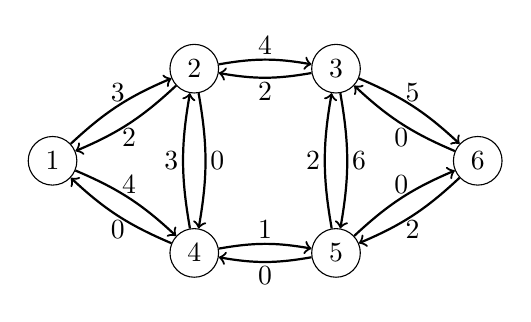
\begin{tikzpicture}[scale=0.9,label distance=-2mm]
\node[draw, circle] (1) at (1,1.3) {$1$};
\node[draw, circle] (2) at (3,2.6) {$2$};
\node[draw, circle] (3) at (5,2.6) {$3$};
\node[draw, circle] (4) at (7,1.3) {$6$};
\node[draw, circle] (5) at (3,0) {$4$};
\node[draw, circle] (6) at (5,0) {$5$};

\path[draw,thick,->] (1) edge [bend left=10] node[font=\small,label=3] {} (2);
\path[draw,thick,->] (2) edge [bend left=10] node[font=\small,label=below:2] {} (1);
\path[draw,thick,->] (2) edge [bend left=10] node[font=\small,label=4] {} (3);
\path[draw,thick,->] (3) edge [bend left=10] node[font=\small,label=below:2] {} (2);
\path[draw,thick,->] (3) edge [bend left=10] node[font=\small,label=5] {} (4);
\path[draw,thick,->] (4) edge [bend left=10] node[font=\small,label=below:0] {} (3);
\path[draw,thick,->] (1) edge [bend left=10] node[font=\small,label=4] {} (5);
\path[draw,thick,->] (5) edge [bend left=10] node[font=\small,label=below:0] {} (1);
\path[draw,thick,->] (5) edge [bend left=10] node[font=\small,label=1] {} (6);
\path[draw,thick,->] (6) edge [bend left=10] node[font=\small,label=below:0] {} (5);
\path[draw,thick,->] (6) edge [bend left=10] node[font=\small,label=0] {} (4);
\path[draw,thick,->] (4) edge [bend left=10] node[font=\small,label=below:2] {} (6);
\path[draw,thick,->] (5) edge [bend left=10] node[font=\small,label=left:3] {} (2);
\path[draw,thick,->] (2) edge [bend left=10] node[font=\small,label=right:0] {} (5);
\path[draw,thick,->] (3) edge [bend left=10] node[font=\small,label=right:6] {} (6);
\path[draw,thick,->] (6) edge [bend left=10] node[font=\small,label=left:2] {} (3);
\end{tikzpicture}
\end{center}

A ideia é que aumentar o fluxo diminui a quantidade de
fluxo que pode passar pelas arestas no futuro.
Por outro lado, é possível cancelar
o fluxo posteriormente usando as arestas reversas do grafo
se isso se mostrar
benéfico para direcionar o fluxo de outra forma.

O algoritmo aumenta o fluxo enquanto
houver um caminho da fonte
para o sumidouro por meio de arestas de peso positivo.
No presente exemplo, nosso próximo caminho pode ser o seguinte:

\begin{center}
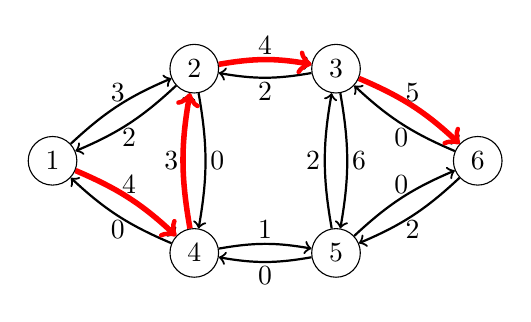
\begin{tikzpicture}[scale=0.9,label distance=-2mm]
\node[draw, circle] (1) at (1,1.3) {$1$};
\node[draw, circle] (2) at (3,2.6) {$2$};
\node[draw, circle] (3) at (5,2.6) {$3$};
\node[draw, circle] (4) at (7,1.3) {$6$};
\node[draw, circle] (5) at (3,0) {$4$};
\node[draw, circle] (6) at (5,0) {$5$};

\path[draw,thick,->] (1) edge [bend left=10] node[font=\small,label=3] {} (2);
\path[draw,thick,->] (2) edge [bend left=10] node[font=\small,label=below:2] {} (1);
\path[draw,thick,->] (2) edge [bend left=10] node[font=\small,label=4] {} (3);
\path[draw,thick,->] (3) edge [bend left=10] node[font=\small,label=below:2] {} (2);
\path[draw,thick,->] (3) edge [bend left=10] node[font=\small,label=5] {} (4);
\path[draw,thick,->] (4) edge [bend left=10] node[font=\small,label=below:0] {} (3);
\path[draw,thick,->] (1) edge [bend left=10] node[font=\small,label=4] {} (5);
\path[draw,thick,->] (5) edge [bend left=10] node[font=\small,label=below:0] {} (1);
\path[draw,thick,->] (5) edge [bend left=10] node[font=\small,label=1] {} (6);
\path[draw,thick,->] (6) edge [bend left=10] node[font=\small,label=below:0] {} (5);
\path[draw,thick,->] (6) edge [bend left=10] node[font=\small,label=0] {} (4);
\path[draw,thick,->] (4) edge [bend left=10] node[font=\small,label=below:2] {} (6);
\path[draw,thick,->] (5) edge [bend left=10] node[font=\small,label=left:3] {} (2);
\path[draw,thick,->] (2) edge [bend left=10] node[font=\small,label=right:0] {} (5);
\path[draw,thick,->] (3) edge [bend left=10] node[font=\small,label=right:6] {} (6);
\path[draw,thick,->] (6) edge [bend left=10] node[font=\small,label=left:2] {} (3);

\path[draw=red,thick,->,line width=2pt] (1) edge [bend left=10] (5);
\path[draw=red,thick,->,line width=2pt] (5) edge [bend left=10] (2);
\path[draw=red,thick,->,line width=2pt] (2) edge [bend left=10] (3);
\path[draw=red,thick,->,line width=2pt] (3) edge [bend left=10] (4);
\end{tikzpicture}
\end{center}

O menor peso de aresta neste caminho é 3,
então o caminho aumenta o fluxo em 3,
e o fluxo total após o processamento do caminho é 5.

\begin{samepage}
O novo grafo será o seguinte:

\begin{center}
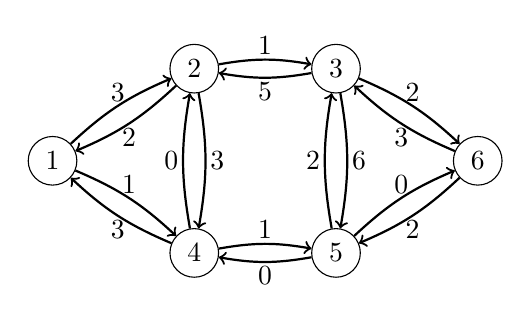
\begin{tikzpicture}[scale=0.9,label distance=-2mm]
\node[draw, circle] (1) at (1,1.3) {$1$};
\node[draw, circle] (2) at (3,2.6) {$2$};
\node[draw, circle] (3) at (5,2.6) {$3$};
\node[draw, circle] (4) at (7,1.3) {$6$};
\node[draw, circle] (5) at (3,0) {$4$};
\node[draw, circle] (6) at (5,0) {$5$};

\path[draw,thick,->] (1) edge [bend left=10] node[font=\small,label=3] {} (2);
\path[draw,thick,->] (2) edge [bend left=10] node[font=\small,label=below:2] {} (1);
\path[draw,thick,->] (2) edge [bend left=10] node[font=\small,label=1] {} (3);
\path[draw,thick,->] (3) edge [bend left=10] node[font=\small,label=below:5] {} (2);
\path[draw,thick,->] (3) edge [bend left=10] node[font=\small,label=2] {} (4);
\path[draw,thick,->] (4) edge [bend left=10] node[font=\small,label=below:3] {} (3);
\path[draw,thick,->] (1) edge [bend left=10] node[font=\small,label=1] {} (5);
\path[draw,thick,->] (5) edge [bend left=10] node[font=\small,label=below:3] {} (1);
\path[draw,thick,->] (5) edge [bend left=10] node[font=\small,label=1] {} (6);
\path[draw,thick,->] (6) edge [bend left=10] node[font=\small,label=below:0] {} (5);
\path[draw,thick,->] (6) edge [bend left=10] node[font=\small,label=0] {} (4);
\path[draw,thick,->] (4) edge [bend left=10] node[font=\small,label=below:2] {} (6);
\path[draw,thick,->] (5) edge [bend left=10] node[font=\small,label=left:0] {} (2);
\path[draw,thick,->] (2) edge [bend left=10] node[font=\small,label=right:3] {} (5);
\path[draw,thick,->] (3) edge [bend left=10] node[font=\small,label=right:6] {} (6);
\path[draw,thick,->] (6) edge [bend left=10] node[font=\small,label=left:2] {} (3);
\end{tikzpicture}
\end{center}
\end{samepage}

Ainda precisamos de mais duas rodadas antes de atingir o fluxo máximo.
Por exemplo, podemos escolher os caminhos
$1 \rightarrow 2 \rightarrow 3 \rightarrow 6$ e
$1 \rightarrow 4 \rightarrow 5 \rightarrow 3 \rightarrow 6$.
Ambos os caminhos aumentam o fluxo em 1,
e o grafo final é o seguinte:

\begin{center}
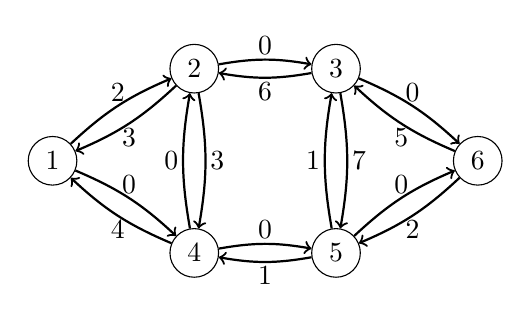
\begin{tikzpicture}[scale=0.9,label distance=-2mm]
\node[draw, circle] (1) at (1,1.3) {$1$};
\node[draw, circle] (2) at (3,2.6) {$2$};
\node[draw, circle] (3) at (5,2.6) {$3$};
\node[draw, circle] (4) at (7,1.3) {$6$};
\node[draw, circle] (5) at (3,0) {$4$};
\node[draw, circle] (6) at (5,0) {$5$};

\path[draw,thick,->] (1) edge [bend left=10] node[font=\small,label=2] {} (2);
\path[draw,thick,->] (2) edge [bend left=10] node[font=\small,label=below:3] {} (1);
\path[draw,thick,->] (2) edge [bend left=10] node[font=\small,label=0] {} (3);
\path[draw,thick,->] (3) edge [bend left=10] node[font=\small,label=below:6] {} (2);
\path[draw,thick,->] (3) edge [bend left=10] node[font=\small,label=0] {} (4);
\path[draw,thick,->] (4) edge [bend left=10] node[font=\small,label=below:5] {} (3);
\path[draw,thick,->] (1) edge [bend left=10] node[font=\small,label=0] {} (5);
\path[draw,thick,->] (5) edge [bend left=10] node[font=\small,label=below:4] {} (1);
\path[draw,thick,->] (5) edge [bend left=10] node[font=\small,label=0] {} (6);
\path[draw,thick,->] (6) edge [bend left=10] node[font=\small,label=below:1] {} (5);
\path[draw,thick,->] (6) edge [bend left=10] node[font=\small,label=0] {} (4);
\path[draw,thick,->] (4) edge [bend left=10] node[font=\small,label=below:2] {} (6);
\path[draw,thick,->] (5) edge [bend left=10] node[font=\small,label=left:0] {} (2);
\path[draw,thick,->] (2) edge [bend left=10] node[font=\small,label=right:3] {} (5);
\path[draw,thick,->] (3) edge [bend left=10] node[font=\small,label=right:7] {} (6);
\path[draw,thick,->] (6) edge [bend left=10] node[font=\small,label=left:1] {} (3);
\end{tikzpicture}
\end{center}

Não é possível aumentar mais o fluxo,
pois não há caminho da fonte
para o sumidouro com arestas de peso positivo.
Portanto, o algoritmo termina e o fluxo máximo é 7.

\subsubsection{Encontrando caminhos}

O algoritmo de Ford–Fulkerson não especifica
como devemos escolher os caminhos que aumentam o fluxo.
De qualquer forma, o algoritmo terminará mais cedo ou mais tarde
e encontrará corretamente o fluxo máximo.
No entanto, a eficiência do algoritmo depende
da maneira como os caminhos são escolhidos.

Uma maneira simples de encontrar caminhos é usar a busca em profundidade.
Geralmente, isso funciona bem, mas no pior caso,
cada caminho só aumenta o fluxo em 1
e o algoritmo é lento.
Felizmente, podemos evitar esta situação
usando uma das seguintes técnicas:

\index{Algoritmo de Edmonds–Karp}

O \key{algoritmo de Edmonds-Karp} \cite{edm72}
escolhe cada caminho de forma que o número de arestas
no caminho seja o menor possível.
Isso pode ser feito utilizando busca em largura
em vez de busca em profundidade para encontrar os caminhos.
Pode-se provar que isso garante que
o fluxo aumente rapidamente e que a complexidade de tempo
do algoritmo seja $O(m^2 n)$.

\index{algoritmo de escalonamento}

O \key{algoritmo de escalonamento} \cite{ahu91} utiliza busca em profundidade
para encontrar caminhos onde o peso de cada aresta seja
pelo menos um valor limite.
Inicialmente, o valor limite é
algum número grande, por exemplo, a soma de todos
os pesos das arestas do grafo.
Sempre que um caminho não puder ser encontrado,
o valor limite é dividido por 2.
A complexidade de tempo do algoritmo é $O(m^2 \log c)$,
onde $c$ é o valor limite inicial.

Na prática, o algoritmo de escalonamento é mais fácil de implementar,
pois a busca em profundidade pode ser utilizada para encontrar os caminhos.
Ambos os algoritmos são eficientes o suficiente para problemas
que normalmente aparecem em competições de programação.

\subsubsection{Cortes mínimos}

\index{corte mínimo}

Verifica-se que, uma vez que o algoritmo de Ford-Fulkerson
encontra um fluxo máximo,
ele também determina um corte mínimo.
Seja $A$ o conjunto de nós
que podem ser alcançados a partir da fonte
usando arestas de peso positivo.
No grafo de exemplo, $A$ contém os nós 1, 2 e 4:

\begin{center}
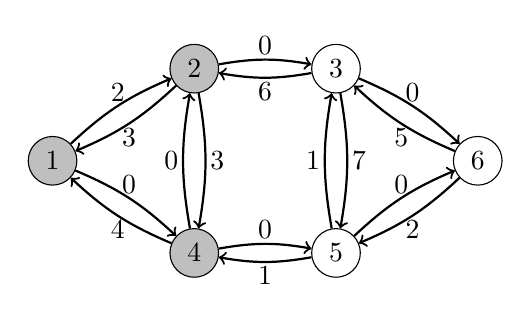
\begin{tikzpicture}[scale=0.9,label distance=-2mm]
\node[draw, circle,fill=lightgray] (1) at (1,1.3) {$1$};
\node[draw, circle,fill=lightgray] (2) at (3,2.6) {$2$};
\node[draw, circle] (3) at (5,2.6) {$3$};
\node[draw, circle] (4) at (7,1.3) {$6$};
\node[draw, circle,fill=lightgray] (5) at (3,0) {$4$};
\node[draw, circle] (6) at (5,0) {$5$};

\path[draw,thick,->] (1) edge [bend left=10] node[font=\small,label=2] {} (2);
\path[draw,thick,->] (2) edge [bend left=10] node[font=\small,label=below:3] {} (1);
\path[draw,thick,->] (2) edge [bend left=10] node[font=\small,label=0] {} (3);
\path[draw,thick,->] (3) edge [bend left=10] node[font=\small,label=below:6] {} (2);
\path[draw,thick,->] (3) edge [bend left=10] node[font=\small,label=0] {} (4);
\path[draw,thick,->] (4) edge [bend left=10] node[font=\small,label=below:5] {} (3);
\path[draw,thick,->] (1) edge [bend left=10] node[font=\small,label=0] {} (5);
\path[draw,thick,->] (5) edge [bend left=10] node[font=\small,label=below:4] {} (1);
\path[draw,thick,->] (5) edge [bend left=10] node[font=\small,label=0] {} (6);
\path[draw,thick,->] (6) edge [bend left=10] node[font=\small,label=below:1] {} (5);
\path[draw,thick,->] (6) edge [bend left=10] node[font=\small,label=0] {} (4);
\path[draw,thick,->] (4) edge [bend left=10] node[font=\small,label=below:2] {} (6);
\path[draw,thick,->] (5) edge [bend left=10] node[font=\small,label=left:0] {} (2);
\path[draw,thick,->] (2) edge [bend left=10] node[font=\small,label=right:3] {} (5);
\path[draw,thick,->] (3) edge [bend left=10] node[font=\small,label=right:7] {} (6);
\path[draw,thick,->] (6) edge [bend left=10] node[font=\small,label=left:1] {} (3);
\end{tikzpicture}
\end{center}

Agora, o corte mínimo consiste nas arestas do grafo original
que começam em algum nó em $A$, terminam em algum nó fora de $A$,
e cuja capacidade é totalmente
utilizada no fluxo máximo.
No grafo acima, tais arestas são
$2 \rightarrow 3$ e $4 \rightarrow 5$,
que correspondem ao corte mínimo $6+1=7$.

Por que o fluxo produzido pelo algoritmo é máximo
e por que o corte é mínimo?
A razão é que um grafo não pode
conter um fluxo cujo tamanho seja maior
que o peso de qualquer corte do grafo.
Portanto, sempre que um fluxo e um corte têm o mesmo tamanho,
eles são um fluxo máximo e um corte mínimo.

Vamos considerar qualquer corte do grafo
tal que a fonte pertença a $A$,
o sumidouro pertença a $B$
e haja algumas arestas entre os conjuntos:

\begin{center}
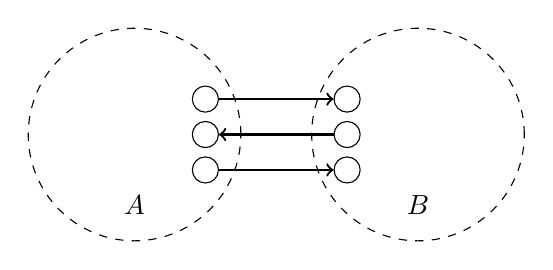
\begin{tikzpicture}[scale=0.9]
\draw[dashed] (-2,0) circle (1.5);
\draw[dashed] (2,0) circle (1.5);

\node at (-2,-1) {$A$};
\node at (2,-1) {$B$};

\node[draw, circle] (1) at (-1,0.5) {};
\node[draw, circle] (2) at (-1,0) {};
\node[draw, circle] (3) at (-1,-0.5) {};
\node[draw, circle] (4) at (1,0.5) {};
\node[draw, circle] (5) at (1,0) {};
\node[draw, circle] (6) at (1,-0.5) {};

\path[draw,thick,->] (1) -- (4);
\path[draw,thick,->] (5) -- (2);
\path[draw,thick,->] (3) -- (6);

\end{tikzpicture}
\end{center}

O tamanho do corte é a soma das arestas
que vão de $A$ para $B$.
Este é um limite superior para o fluxo
no grafo, pois o fluxo precisa prosseguir
de $A$ para $B$.
Assim, o tamanho de um fluxo máximo é menor ou igual a
o tamanho de qualquer corte no grafo.

Por outro lado, o algoritmo de Ford-Fulkerson
produz um fluxo cujo tamanho é \emph{exatamente} igual
ao tamanho de um corte no grafo.
Assim, o fluxo precisa ser um fluxo máximo
e o corte precisa ser um corte mínimo.

\section{Caminhos disjuntos}

Muitos problemas de grafos podem ser resolvidos reduzindo-os
ao problema do fluxo máximo.
Nosso primeiro exemplo de tal problema é
o seguinte: recebemos um grafo direcionado
com uma fonte e um sumidouro,
e nossa tarefa é encontrar o número máximo
de caminhos disjuntos da fonte ao sumidouro.

\subsubsection{Caminhos Disjuntos nas Arestas}

Vamos primeiro focar no problema de
encontrar o número máximo de
\key{caminhos disjuntos nas arestas} da origem ao sumidouro.
Isso significa que devemos construir um conjunto de caminhos
de forma que cada aresta apareça em, no máximo, um caminho.

Por exemplo, considere o seguinte grafo:
\begin{center}
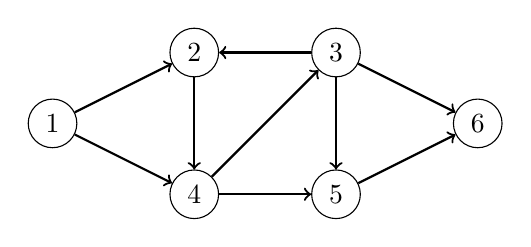
\begin{tikzpicture}[scale=0.9]
\node[draw, circle] (1) at (1,2) {$1$};
\node[draw, circle] (2) at (3,3) {$2$};
\node[draw, circle] (3) at (5,3) {$3$};
\node[draw, circle] (4) at (3,1) {$4$};
\node[draw, circle] (5) at (5,1) {$5$};
\node[draw, circle] (6) at (7,2) {$6$};
\path[draw,thick,->] (1) -- (2);
\path[draw,thick,->] (1) -- (4);
\path[draw,thick,->] (2) -- (4);
\path[draw,thick,->] (3) -- (2);
\path[draw,thick,->] (3) -- (5);
\path[draw,thick,->] (3) -- (6);
\path[draw,thick,->] (4) -- (3);
\path[draw,thick,->] (4) -- (5);
\path[draw,thick,->] (5) -- (6);
\end{tikzpicture}
\end{center}

Neste grafo, o número máximo de caminhos disjuntos nas arestas é 2.
Podemos escolher os caminhos
$1 \rightarrow 2 \rightarrow 4 \rightarrow 3 \rightarrow 6$
e $1 \rightarrow 4 \rightarrow 5 \rightarrow 6$ como segue:

\begin{center}
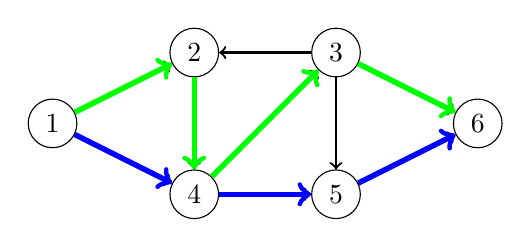
\begin{tikzpicture}[scale=0.9]
\node[draw, circle] (1) at (1,2) {$1$};
\node[draw, circle] (2) at (3,3) {$2$};
\node[draw, circle] (3) at (5,3) {$3$};
\node[draw, circle] (4) at (3,1) {$4$};
\node[draw, circle] (5) at (5,1) {$5$};
\node[draw, circle] (6) at (7,2) {$6$};
\path[draw,thick,->] (1) -- (2);
\path[draw,thick,->] (1) -- (4);
\path[draw,thick,->] (2) -- (4);
\path[draw,thick,->] (3) -- (2);
\path[draw,thick,->] (3) -- (5);
\path[draw,thick,->] (3) -- (6);
\path[draw,thick,->] (4) -- (3);
\path[draw,thick,->] (4) -- (5);
\path[draw,thick,->] (5) -- (6);

\path[draw=green,thick,->,line width=2pt] (1) -- (2);
\path[draw=green,thick,->,line width=2pt] (2) -- (4);
\path[draw=green,thick,->,line width=2pt] (4) -- (3);
\path[draw=green,thick,->,line width=2pt] (3) -- (6);

\path[draw=blue,thick,->,line width=2pt] (1) -- (4);
\path[draw=blue,thick,->,line width=2pt] (4) -- (5);
\path[draw=blue,thick,->,line width=2pt] (5) -- (6);
\end{tikzpicture}
\end{center}

Verifica-se que o número máximo de
caminhos disjuntos nas arestas
é igual ao fluxo máximo do grafo,
assumindo que a capacidade de cada aresta é um.
Depois que o fluxo máximo é construído,
os caminhos disjuntos nas arestas podem ser encontrados avidamente
seguindo os caminhos da origem ao sumidouro.

\subsubsection{Caminhos Disjuntos nos Vértices}

Agora vamos considerar outro problema:
encontrar o número máximo de
\key{caminhos disjuntos nos vértices} da origem
ao sumidouro.
Neste problema, cada vértice,
exceto a origem e o sumidouro,
pode aparecer em, no máximo, um caminho.
O número de caminhos disjuntos nos vértices
pode ser menor que o número de
caminhos disjuntos nas arestas.

Por exemplo, no grafo anterior,
o número máximo de caminhos disjuntos nos vértices é 1:

\begin{center}
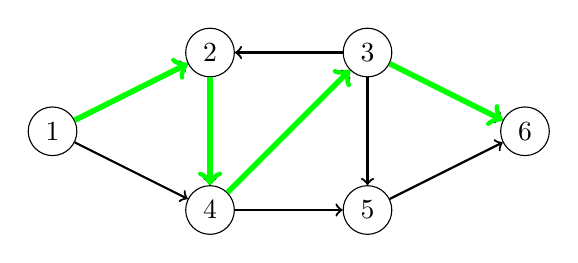
\begin{tikzpicture}
\node[draw, circle] (1) at (1,2) {$1$};
\node[draw, circle] (2) at (3,3) {$2$};
\node[draw, circle] (3) at (5,3) {$3$};
\node[draw, circle] (4) at (3,1) {$4$};
\node[draw, circle] (5) at (5,1) {$5$};
\node[draw, circle] (6) at (7,2) {$6$};
\path[draw,thick,->] (1) -- (2);
\path[draw,thick,->] (1) -- (4);
\path[draw,thick,->] (2) -- (4);
\path[draw,thick,->] (3) -- (2);
\path[draw,thick,->] (3) -- (5);
\path[draw,thick,->] (3) -- (6);
\path[draw,thick,->] (4) -- (3);
\path[draw,thick,->] (4) -- (5);
\path[draw,thick,->] (5) -- (6);

\path[draw=green,thick,->,line width=2pt] (1) -- (2);
\path[draw=green,thick,->,line width=2pt] (2) -- (4);
\path[draw=green,thick,->,line width=2pt] (4) -- (3);
\path[draw=green,thick,->,line width=2pt] (3) -- (6);
\end{tikzpicture}
\end{center}

Também podemos reduzir este problema ao problema do fluxo máximo.
Como cada vértice pode aparecer em, no máximo, um caminho,
temos que limitar o fluxo que passa pelos vértices.
Um método padrão para isso é dividir cada vértice em
dois vértices, de forma que o primeiro vértice tenha as arestas de entrada
do vértice original, o segundo vértice tenha as arestas de saída
do vértice original e
haja uma nova aresta do primeiro vértice
para o segundo vértice.

No nosso exemplo, o grafo se torna o seguinte:
\begin{center}
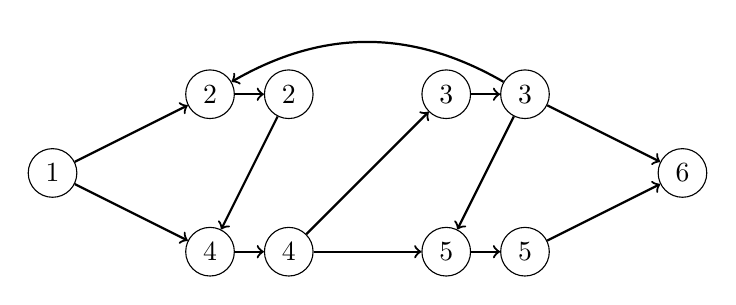
\begin{tikzpicture}
\node[draw, circle] (1) at (1,2) {$1$};

\node[draw, circle] (2a) at (3,3) {$2$};
\node[draw, circle] (3a) at (6,3) {$3$};
\node[draw, circle] (4a) at (3,1) {$4$};
\node[draw, circle] (5a) at (6,1) {$5$};

\node[draw, circle] (2b) at (4,3) {$2$};
\node[draw, circle] (3b) at (7,3) {$3$};
\node[draw, circle] (4b) at (4,1) {$4$};
\node[draw, circle] (5b) at (7,1) {$5$};

\node[draw, circle] (6) at (9,2) {$6$};

\path[draw,thick,->] (2a) -- (2b);
\path[draw,thick,->] (3a) -- (3b);
\path[draw,thick,->] (4a) -- (4b);
\path[draw,thick,->] (5a) -- (5b);

\path[draw,thick,->] (1) -- (2a);
\path[draw,thick,->] (1) -- (4a);
\path[draw,thick,->] (2b) -- (4a);
\path[draw,thick,->] (3b) edge [bend right=30] (2a);
\path[draw,thick,->] (3b) -- (5a);
\path[draw,thick,->] (3b) -- (6);
\path[draw,thick,->] (4b) -- (3a);
\path[draw,thick,->] (4b) -- (5a);
\path[draw,thick,->] (5b) -- (6);
\end{tikzpicture}
\end{center}

O fluxo máximo para o grafo é o seguinte:
\begin{center}
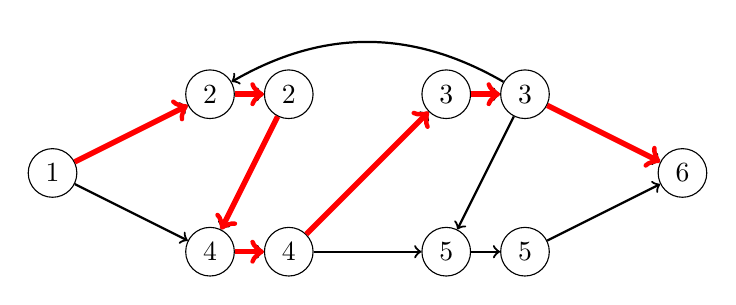
\begin{tikzpicture}
\node[draw, circle] (1) at (1,2) {$1$};

\node[draw, circle] (2a) at (3,3) {$2$};
\node[draw, circle] (3a) at (6,3) {$3$};
\node[draw, circle] (4a) at (3,1) {$4$};
\node[draw, circle] (5a) at (6,1) {$5$};

\node[draw, circle] (2b) at (4,3) {$2$};
\node[draw, circle] (3b) at (7,3) {$3$};
\node[draw, circle] (4b) at (4,1) {$4$};
\node[draw, circle] (5b) at (7,1) {$5$};

\node[draw, circle] (6) at (9,2) {$6$};

\path[draw,thick,->] (2a) -- (2b);
\path[draw,thick,->] (3a) -- (3b);
\path[draw,thick,->] (4a) -- (4b);
\path[draw,thick,->] (5a) -- (5b);

\path[draw,thick,->] (1) -- (2a);
\path[draw,thick,->] (1) -- (4a);
\path[draw,thick,->] (2b) -- (4a);
\path[draw,thick,->] (3b) edge [bend right=30] (2a);
\path[draw,thick,->] (3b) -- (5a);
\path[draw,thick,->] (3b) -- (6);
\path[draw,thick,->] (4b) -- (3a);
\path[draw,thick,->] (4b) -- (5a);
\path[draw,thick,->] (5b) -- (6);

\path[draw=red,thick,->,line width=2pt] (1) -- (2a);
\path[draw=red,thick,->,line width=2pt] (2a) -- (2b);
\path[draw=red,thick,->,line width=2pt] (2b) -- (4a);
\path[draw=red,thick,->,line width=2pt] (4a) -- (4b);
\path[draw=red,thick,->,line width=2pt] (4b) -- (3a);
\path[draw=red,thick,->,line width=2pt] (3a) -- (3b);
\path[draw=red,thick,->,line width=2pt] (3b) -- (6);
\end{tikzpicture}
\end{center}

Assim, o número máximo de caminhos disjuntos nos vértices
da origem ao sumidouro é 1.

\section{Emparelhamentos Máximos}

\index{emparelhamento}
\index{emparelhamento máximo}

O problema do \key{emparelhamento máximo} pede para encontrar
um conjunto de tamanho máximo de pares de vértices em um grafo não direcionado,
de forma que cada par esteja conectado por uma aresta e
cada vértice pertença a, no máximo, um par.

Existem algoritmos polinomiais para encontrar
emparelhamentos máximos em grafos gerais \cite{edm65},
mas tais algoritmos são complexos e
raramente vistos em competições de programação.
No entanto, em grafos bipartidos,
o problema do emparelhamento máximo é muito mais fácil
de resolver, porque podemos reduzi-lo ao
problema do fluxo máximo.

\subsubsection{Encontrando Emparelhamentos Máximos}

Os vértices de um grafo bipartido sempre podem
ser divididos em dois grupos, de forma que todas as arestas
do grafo vão do grupo esquerdo para o grupo direito.
Por exemplo, no seguinte grafo bipartido,
os grupos são $\{1,2,3,4\}$ e $\{5,6,7,8\}$.

\begin{center}
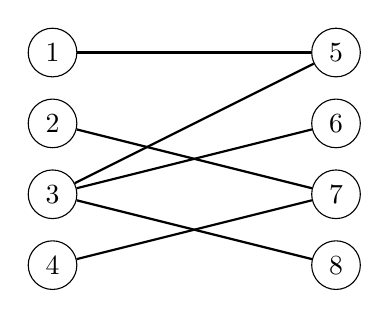
\begin{tikzpicture}[scale=0.60]
\node[draw, circle] (1) at (2,4.5) {1};
\node[draw, circle] (2) at (2,3) {2};
\node[draw, circle] (3) at (2,1.5) {3};
\node[draw, circle] (4) at (2,0) {4};
\node[draw, circle] (5) at (8,4.5) {5};
\node[draw, circle] (6) at (8,3) {6};
\node[draw, circle] (7) at (8,1.5) {7};
\node[draw, circle] (8) at (8,0) {8};

\path[draw,thick,-] (1) -- (5);
\path[draw,thick,-] (2) -- (7);
\path[draw,thick,-] (3) -- (5);
\path[draw,thick,-] (3) -- (6);
\path[draw,thick,-] (3) -- (8);
\path[draw,thick,-] (4) -- (7);
\end{tikzpicture}
\end{center}
O tamanho de um emparelhamento máximo deste grafo é 3:
\begin{center}
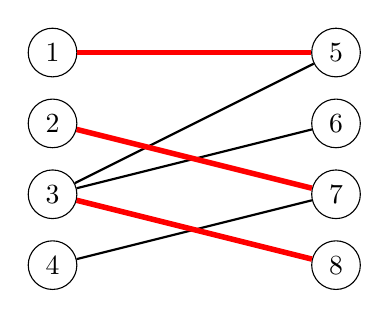
\begin{tikzpicture}[scale=0.60]
\node[draw, circle] (1) at (2,4.5) {1};
\node[draw, circle] (2) at (2,3) {2};
\node[draw, circle] (3) at (2,1.5) {3};
\node[draw, circle] (4) at (2,0) {4};
\node[draw, circle] (5) at (8,4.5) {5};
\node[draw, circle] (6) at (8,3) {6};
\node[draw, circle] (7) at (8,1.5) {7};
\node[draw, circle] (8) at (8,0) {8};

\path[draw,thick,-] (1) -- (5);
\path[draw,thick,-] (2) -- (7);
\path[draw,thick,-] (3) -- (5);
\path[draw,thick,-] (3) -- (6);
\path[draw,thick,-] (3) -- (8);
\path[draw,thick,-] (4) -- (7);

\path[draw=red,thick,-,line width=2pt] (1) -- (5);
\path[draw=red,thick,-,line width=2pt] (2) -- (7);
\path[draw=red,thick,-,line width=2pt] (3) -- (8);
\end{tikzpicture}
\end{center}

Podemos reduzir o problema do emparelhamento máximo bipartido
ao problema do fluxo máximo adicionando dois novos vértices
ao grafo: uma origem e um sumidouro.
Também adicionamos arestas da origem
para cada vértice esquerdo e de cada vértice direito para o sumidouro.
Depois disso, o tamanho de um fluxo máximo no grafo
é igual ao tamanho de um emparelhamento máximo no grafo original.

Por exemplo, a redução para o grafo acima
é a seguinte:
\begin{center}
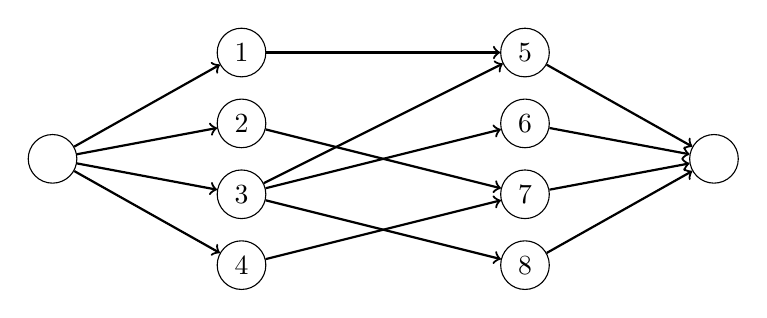
\begin{tikzpicture}[scale=0.60]
\node[draw, circle] (1) at (2,4.5) {1};
\node[draw, circle] (2) at (2,3) {2};
\node[draw, circle] (3) at (2,1.5) {3};
\node[draw, circle] (4) at (2,0) {4};
\node[draw, circle] (5) at (8,4.5) {5};
\node[draw, circle] (6) at (8,3) {6};
\node[draw, circle] (7) at (8,1.5) {7};
\node[draw, circle] (8) at (8,0) {8};

\node[draw, circle] (a) at (-2,2.25) {\phantom{0}};
\node[draw, circle] (b) at (12,2.25) {\phantom{0}};

\path[draw,thick,->] (1) -- (5);
\path[draw,thick,->] (2) -- (7);
\path[draw,thick,->] (3) -- (5);
\path[draw,thick,->] (3) -- (6);
\path[draw,thick,->] (3) -- (8);
\path[draw,thick,->] (4) -- (7);

\path[draw,thick,->] (a) -- (1);
\path[draw,thick,->] (a) -- (2);
\path[draw,thick,->] (a) -- (3);
\path[draw,thick,->] (a) -- (4);
\path[draw,thick,->] (5) -- (b);
\path[draw,thick,->] (6) -- (b);
\path[draw,thick,->] (7) -- (b);
\path[draw,thick,->] (8) -- (b);
\end{tikzpicture}
\end{center}

O fluxo máximo deste grafo é o seguinte:
\begin{center}
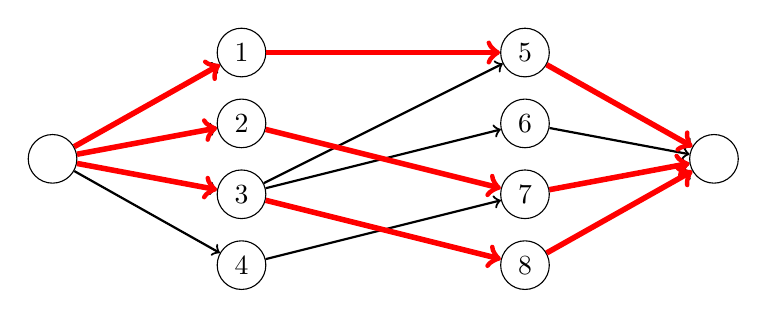
\begin{tikzpicture}[scale=0.60]
\node[draw, circle] (1) at (2,4.5) {1};
\node[draw, circle] (2) at (2,3) {2};
\node[draw, circle] (3) at (2,1.5) {3};
\node[draw, circle] (4) at (2,0) {4};
\node[draw, circle] (5) at (8,4.5) {5};
\node[draw, circle] (6) at (8,3) {6};
\node[draw, circle] (7) at (8,1.5) {7};
\node[draw, circle] (8) at (8,0) {8};

\node[draw, circle] (a) at (-2,2.25) {\phantom{0}};
\node[draw, circle] (b) at (12,2.25) {\phantom{0}};

\path[draw,thick,->] (3) -- (5);
\path[draw,thick,->] (3) -- (6);
\path[draw,thick,->] (4) -- (7);

\path[draw,thick,->] (a) -- (1);
\path[draw,thick,->] (a) -- (2);
\path[draw,thick,->] (a) -- (3);
\path[draw,thick,->] (a) -- (4);
\path[draw,thick,->] (5) -- (b);
\path[draw,thick,->] (6) -- (b);
\path[draw,thick,->] (7) -- (b);
\path[draw,thick,->] (8) -- (b);

\path[draw=red,thick,->,line width=2pt] (1) -- (5);
\path[draw=red,thick,->,line width=2pt] (2) -- (7);
\path[draw=red,thick,->,line width=2pt] (3) -- (8);

\path[draw=red,thick,->,line width=2pt] (a) -- (1);
\path[draw=red,thick,->,line width=2pt] (a) -- (2);
\path[draw=red,thick,->,line width=2pt] (a) -- (3);

\path[draw=red,thick,->,line width=2pt] (5) -- (b);
\path[draw=red,thick,->,line width=2pt] (7) -- (b);
\path[draw=red,thick,->,line width=2pt] (8) -- (b);

\end{tikzpicture}
\end{center}

\subsubsection{Teorema de Hall}

\index{Teorema de Hall}
\index{emparelhamento perfeito}

O \key{Teorema de Hall} pode ser usado para descobrir
se um grafo bipartido possui um emparelhamento
que contém todos os vértices esquerdos ou direitos.
Se o número de vértices esquerdos e direitos for o mesmo,
o Teorema de Hall nos diz se é possível
construir um \key{emparelhamento perfeito} que
contenha todos os vértices do grafo.

Assuma que queremos encontrar um emparelhamento
que contenha todos os vértices esquerdos.
Seja $X$ qualquer conjunto de vértices esquerdos
e seja $f(X)$ o conjunto de seus vizinhos.
De acordo com o Teorema de Hall, um emparelhamento
que contém todos os vértices esquerdos existe
exatamente quando, para cada $X$, a condição $|X| \le |f(X)|$ é válida.

Vamos estudar o Teorema de Hall no grafo de exemplo.
Primeiro, seja $X=\{1,3\}$ o que produz$f(X)=\{5,6,8\}$:

\begin{center}
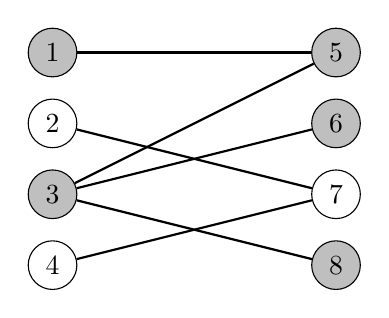
\begin{tikzpicture}[scale=0.60]
\node[draw, circle, fill=lightgray] (1) at (2,4.5) {1};
\node[draw, circle] (2) at (2,3) {2};
\node[draw, circle, fill=lightgray] (3) at (2,1.5) {3};
\node[draw, circle] (4) at (2,0) {4};
\node[draw, circle, fill=lightgray] (5) at (8,4.5) {5};
\node[draw, circle, fill=lightgray] (6) at (8,3) {6};
\node[draw, circle] (7) at (8,1.5) {7};
\node[draw, circle, fill=lightgray] (8) at (8,0) {8};

\path[draw,thick,-] (1) -- (5);
\path[draw,thick,-] (2) -- (7);
\path[draw,thick,-] (3) -- (5);
\path[draw,thick,-] (3) -- (6);
\path[draw,thick,-] (3) -- (8);
\path[draw,thick,-] (4) -- (7);
\end{tikzpicture}
\end{center}

A condição do Teorema de Hall é válida, pois
$|X|=2$ e $|f(X)|=3$.
Em seguida, seja $X=\{2,4\}$ o que produz $f(X)=\{7\}$:

\begin{center}
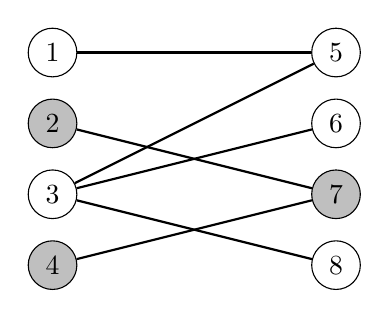
\begin{tikzpicture}[scale=0.60]
\node[draw, circle] (1) at (2,4.5) {1};
\node[draw, circle, fill=lightgray] (2) at (2,3) {2};
\node[draw, circle] (3) at (2,1.5) {3};
\node[draw, circle, fill=lightgray] (4) at (2,0) {4};
\node[draw, circle] (5) at (8,4.5) {5};
\node[draw, circle] (6) at (8,3) {6};
\node[draw, circle, fill=lightgray] (7) at (8,1.5) {7};
\node[draw, circle] (8) at (8,0) {8};

\path[draw,thick,-] (1) -- (5);
\path[draw,thick,-] (2) -- (7);
\path[draw,thick,-] (3) -- (5);
\path[draw,thick,-] (3) -- (6);
\path[draw,thick,-] (3) -- (8);
\path[draw,thick,-] (4) -- (7);
\end{tikzpicture}
\end{center}

Neste caso, $|X|=2$ e $|f(X)|=1$,
então a condição do Teorema de Hall não é válida.
Isso significa que não é possível formar
um emparelhamento perfeito para o grafo.
Este resultado não é surpreendente, porque já
sabemos que o emparelhamento máximo do grafo é 3 e não 4.

Se a condição do Teorema de Hall não for válida,
o conjunto $X$ fornece uma explicação \emph{por que}
não podemos formar tal emparelhamento.
Como $X$ contém mais vértices do que $f(X)$,
não há pares para todos os vértices em $X$.
Por exemplo, no grafo acima, ambos os vértices 2 e 4
deveriam ser conectados ao vértice 7, o que não é possível.

\subsubsection{Teorema de Kőnig}

\index{Teorema de Kőnig}
\index{cobertura por vértices}
\index{cobertura mínima por vértices}

Uma \key{cobertura mínima por vértices} de um grafo
é um conjunto mínimo de vértices, de forma que cada aresta do grafo
tenha pelo menos um vértice no conjunto.
Em um grafo geral, encontrar uma cobertura mínima por vértices
é um problema NP-difícil.
No entanto, se o grafo for bipartido,
o \key{Teorema de Kőnig} nos diz que
o tamanho de uma cobertura mínima por vértices
e o tamanho de um emparelhamento máximo são sempre iguais.
Assim, podemos calcular o tamanho de uma cobertura mínima por vértices
usando um algoritmo de fluxo máximo.

Vamos considerar o seguinte grafo
com um emparelhamento máximo de tamanho 3:
\begin{center}
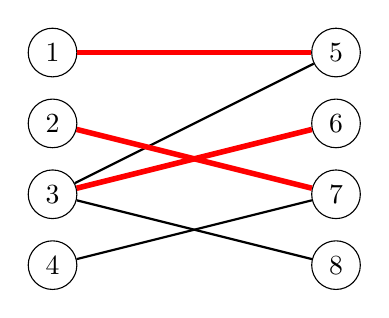
\begin{tikzpicture}[scale=0.60]
\node[draw, circle] (1) at (2,4.5) {1};
\node[draw, circle] (2) at (2,3) {2};
\node[draw, circle] (3) at (2,1.5) {3};
\node[draw, circle] (4) at (2,0) {4};
\node[draw, circle] (5) at (8,4.5) {5};
\node[draw, circle] (6) at (8,3) {6};
\node[draw, circle] (7) at (8,1.5) {7};
\node[draw, circle] (8) at (8,0) {8};

\path[draw,thick,-] (1) -- (5);
\path[draw,thick,-] (2) -- (7);
\path[draw,thick,-] (3) -- (5);
\path[draw,thick,-] (3) -- (6);
\path[draw,thick,-] (3) -- (8);
\path[draw,thick,-] (4) -- (7);

\path[draw=red,thick,-,line width=2pt] (1) -- (5);
\path[draw=red,thick,-,line width=2pt] (2) -- (7);
\path[draw=red,thick,-,line width=2pt] (3) -- (6);
\end{tikzpicture}
\end{center}
Agora, o Teorema de Kőnig nos diz que o tamanho
de uma cobertura mínima por vértices também é 3.
Tal cobertura pode ser construída da seguinte forma:

\begin{center}
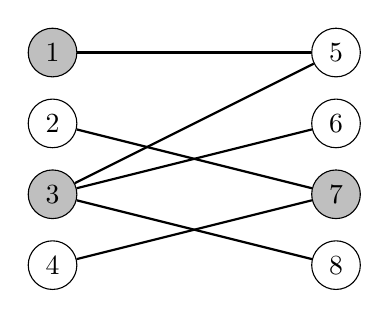
\begin{tikzpicture}[scale=0.60]
\node[draw, circle, fill=lightgray] (1) at (2,4.5) {1};
\node[draw, circle] (2) at (2,3) {2};
\node[draw, circle, fill=lightgray] (3) at (2,1.5) {3};
\node[draw, circle] (4) at (2,0) {4};
\node[draw, circle] (5) at (8,4.5) {5};
\node[draw, circle] (6) at (8,3) {6};
\node[draw, circle, fill=lightgray] (7) at (8,1.5) {7};
\node[draw, circle] (8) at (8,0) {8};

\path[draw,thick,-] (1) -- (5);
\path[draw,thick,-] (2) -- (7);
\path[draw,thick,-] (3) -- (5);
\path[draw,thick,-] (3) -- (6);
\path[draw,thick,-] (3) -- (8);
\path[draw,thick,-] (4) -- (7);
\end{tikzpicture}
\end{center}

\index{conjunto independente}
\index{conjunto independente máximo}

Os vértices que \emph{não}
pertencem a uma cobertura mínima por vértices
formam um \key{conjunto independente máximo}.
Este é o maior conjunto possível de vértices,
de forma que não haja dois vértices no conjunto
que estejam conectados por uma aresta.
Mais uma vez, encontrar um conjunto independente máximo
em um grafo geral é um problema NP-difícil,
mas, em um grafo bipartido, podemos usar
o Teorema de Kőnig para resolver o problema de forma eficiente.
No grafo de exemplo, o conjunto independente máximo
é o seguinte:

\begin{center}
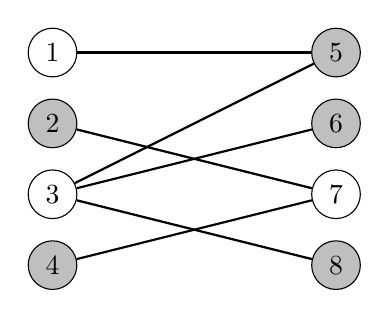
\begin{tikzpicture}[scale=0.60]
\node[draw, circle] (1) at (2,4.5) {1};
\node[draw, circle, fill=lightgray] (2) at (2,3) {2};
\node[draw, circle] (3) at (2,1.5) {3};
\node[draw, circle, fill=lightgray] (4) at (2,0) {4};
\node[draw, circle, fill=lightgray] (5) at (8,4.5) {5};
\node[draw, circle, fill=lightgray] (6) at (8,3) {6};
\node[draw, circle] (7) at (8,1.5) {7};
\node[draw, circle, fill=lightgray] (8) at (8,0) {8};

\path[draw,thick,-] (1) -- (5);
\path[draw,thick,-] (2) -- (7);
\path[draw,thick,-] (3) -- (5);
\path[draw,thick,-] (3) -- (6);
\path[draw,thick,-] (3) -- (8);
\path[draw,thick,-] (4) -- (7);
\end{tikzpicture}
\end{center}

\section{Coberturas por Caminhos}

\index{cobertura por caminhos}

Uma \key{cobertura por caminhos} é um conjunto de caminhos em um grafo,
de forma que cada vértice do grafo pertença a pelo menos um caminho.
Acontece que, em grafos direcionados acíclicos,
podemos reduzir o problema de encontrar uma cobertura mínima por caminhos
ao problema de encontrar um fluxo máximo em outro grafo.

\subsubsection{Cobertura por Caminhos Disjuntos nos Vértices}

Em uma \key{cobertura por caminhos disjuntos nos vértices},
cada vértice pertence a exatamente um caminho.
Como exemplo, considere o seguinte grafo:
\begin{center}
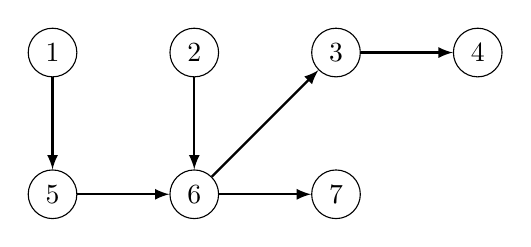
\begin{tikzpicture}[scale=0.9]
\node[draw, circle] (1) at (0,0) {1};
\node[draw, circle] (2) at (2,0) {2};
\node[draw, circle] (3) at (4,0) {3};
\node[draw, circle] (4) at (6,0) {4};
\node[draw, circle] (5) at (0,-2) {5};
\node[draw, circle] (6) at (2,-2) {6};
\node[draw, circle] (7) at (4,-2) {7};

\path[draw,thick,->,>=latex] (1) -- (5);
\path[draw,thick,->,>=latex] (2) -- (6);
\path[draw,thick,->,>=latex] (3) -- (4);
\path[draw,thick,->,>=latex] (5) -- (6);
\path[draw,thick,->,>=latex] (6) -- (3);
\path[draw,thick,->,>=latex] (6) -- (7);
\end{tikzpicture}
\end{center}

Uma cobertura mínima por caminhos disjuntos nos vértices
deste grafo
consiste em três caminhos.
Por exemplo, podemos escolher os seguintes caminhos:

\begin{center}
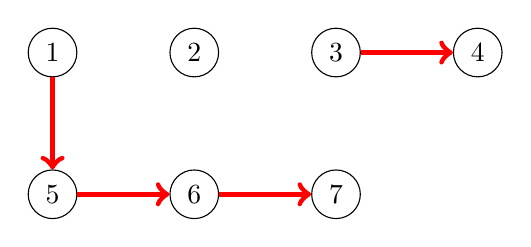
\begin{tikzpicture}[scale=0.9]
\node[draw, circle] (1) at (0,0) {1};
\node[draw, circle] (2) at (2,0) {2};
\node[draw, circle] (3) at (4,0) {3};
\node[draw, circle] (4) at (6,0) {4};
\node[draw, circle] (5) at (0,-2) {5};
\node[draw, circle] (6) at (2,-2) {6};
\node[draw, circle] (7) at (4,-2) {7};

\path[draw=red,thick,->,line width=2pt] (1) -- (5);
\path[draw=red,thick,->,line width=2pt] (5) -- (6);
\path[draw=red,thick,->,line width=2pt] (6) -- (7);
\path[draw=red,thick,->,line width=2pt] (3) -- (4);
\end{tikzpicture}
\end{center}

Observe que um dos caminhos contém apenas o vértice 2,
então é possível que um caminho não contenha nenhuma aresta.

Podemos encontrar uma cobertura mínima por caminhos disjuntos nos vértices
construindo um \emph{grafo de emparelhamento}, onde cada vértice
do grafo original é representado por
dois vértices: um vértice esquerdo e um vértice direito.
Há uma aresta de um vértice esquerdo para um vértice direito
se houver tal aresta no grafo original.
Além disso, o grafo de emparelhamento contém uma origem e um sumidouro,
e há arestas da origem para todos
os vértices esquerdos e de todos os vértices direitos para o sumidouro.

Um emparelhamento máximo no grafo resultante corresponde
a uma cobertura mínima por caminhos disjuntos nos vértices no
grafo original.
Por exemplo, o seguinte grafo de emparelhamento
para o grafo acima contém
um emparelhamento máximo de tamanho 4:

\begin{center}
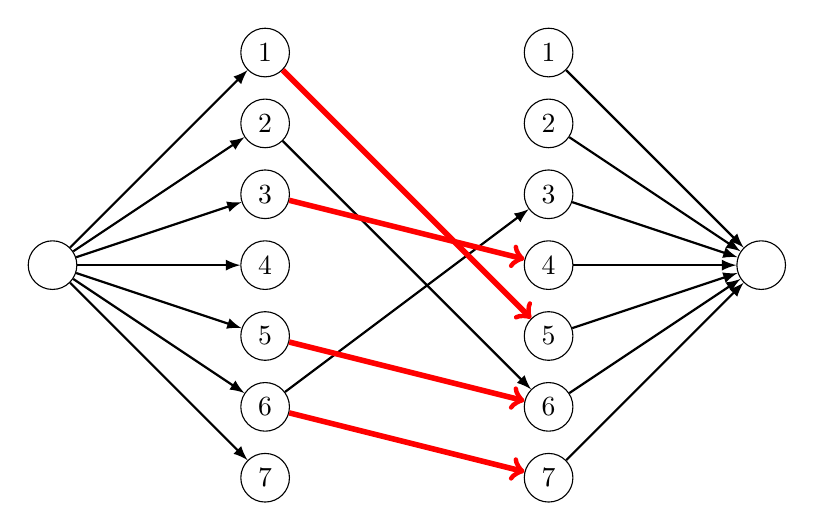
\begin{tikzpicture}[scale=0.9]
\node[draw, circle] (1a) at (0,6) {1};
\node[draw, circle] (2a) at (0,5) {2};
\node[draw, circle] (3a) at (0,4) {3};
\node[draw, circle] (4a) at (0,3) {4};
\node[draw, circle] (5a) at (0,2) {5};
\node[draw, circle] (6a) at (0,1) {6};
\node[draw, circle] (7a) at (0,0) {7};

\node[draw, circle] (1b) at (4,6) {1};
\node[draw, circle] (2b) at (4,5) {2};
\node[draw, circle] (3b) at (4,4) {3};
\node[draw, circle] (4b) at (4,3) {4};
\node[draw, circle] (5b) at (4,2) {5};
\node[draw, circle] (6b) at (4,1) {6};
\node[draw, circle] (7b) at (4,0) {7};

\node[draw, circle] (a) at (-3,3) {\phantom{0}};
\node[draw, circle] (b) at (7,3) {\phantom{0}};

%\path[draw,thick,->,>=latex] (1a) -- (5b);
\path[draw,thick,->,>=latex] (2a) -- (6b);
%\path[draw,thick,->,>=latex] (3a) -- (4b);
%\path[draw,thick,->,>=latex] (5a) -- (6b);
\path[draw,thick,->,>=latex] (6a) -- (3b);
%\path[draw,thick,->,>=latex] (6a) -- (7b);

\path[draw,thick,->,>=latex] (a) -- (1a);
\path[draw,thick,->,>=latex] (a) -- (2a);
\path[draw,thick,->,>=latex] (a) -- (3a);
\path[draw,thick,->,>=latex] (a) -- (4a);
\path[draw,thick,->,>=latex] (a) -- (5a);
\path[draw,thick,->,>=latex] (a) -- (6a);
\path[draw,thick,->,>=latex] (a) -- (7a);

\path[draw,thick,->,>=latex] (1b) -- (b);
\path[draw,thick,->,>=latex] (2b) -- (b);
\path[draw,thick,->,>=latex] (3b) -- (b);
\path[draw,thick,->,>=latex] (4b) -- (b);
\path[draw,thick,->,>=latex] (5b) -- (b);
\path[draw,thick,->,>=latex] (6b) -- (b);
\path[draw,thick,->,>=latex] (7b) -- (b);

\path[draw=red,thick,->,line width=2pt] (1a) -- (5b);
\path[draw=red,thick,->,line width=2pt] (5a) -- (6b);
\path[draw=red,thick,->,line width=2pt] (6a) -- (7b);
\path[draw=red,thick,->,line width=2pt] (3a) -- (4b);

\end{tikzpicture}
\end{center}

Cada aresta no emparelhamento máximo do grafo de emparelhamento corresponde
a uma aresta na cobertura mínima por caminhos disjuntos nos vértices
do grafo original.
Assim, o tamanho da cobertura mínima por caminhos disjuntos nos vértices é $n-c$,
onde $n$ é o número de vértices no grafo original
e $c$ é o tamanho do emparelhamento máximo.

\subsubsection{Cobertura Geral por Caminhos}

Uma \key{cobertura geral por caminhos} é uma cobertura por caminhos
onde um vértice pode pertencer a mais de um caminho.
Uma cobertura geral mínima por caminhos pode ser menor
que uma cobertura mínima por caminhos disjuntos nos vértices,
porque um vértice pode ser usado várias vezes em caminhos.
Considere novamente o seguinte grafo:
\begin{center}
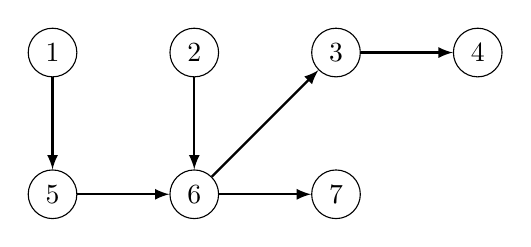
\begin{tikzpicture}[scale=0.9]
\node[draw, circle] (1) at (0,0) {1};
\node[draw, circle] (2) at (2,0) {2};
\node[draw, circle] (3) at (4,0) {3};
\node[draw, circle] (4) at (6,0) {4};
\node[draw, circle] (5) at (0,-2) {5};
\node[draw, circle] (6) at (2,-2) {6};
\node[draw, circle] (7) at (4,-2) {7};

\path[draw,thick,->,>=latex] (1) -- (5);
\path[draw,thick,->,>=latex] (2) -- (6);
\path[draw,thick,->,>=latex] (3) -- (4);
\path[draw,thick,->,>=latex] (5) -- (6);
\path[draw,thick,->,>=latex] (6) -- (3);
\path[draw,thick,->,>=latex] (6) -- (7);
\end{tikzpicture}
\end{center}

A cobertura geral mínima por caminhos deste grafo
consiste em dois caminhos.
Por exemplo, o primeiro caminho pode ser o seguinte:
\begin{center}
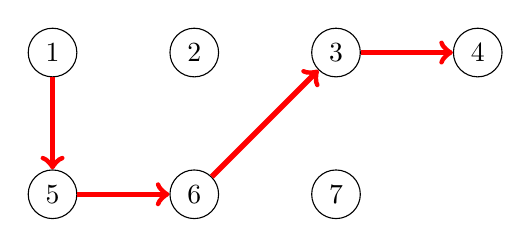
\begin{tikzpicture}[scale=0.9]
\node[draw, circle] (1) at (0,0) {1};
\node[draw, circle] (2) at (2,0) {2};
\node[draw, circle] (3) at (4,0) {3};
\node[draw, circle] (4) at (6,0) {4};
\node[draw, circle] (5) at (0,-2) {5};
\node[draw, circle] (6) at (2,-2) {6};
\node[draw, circle] (7) at (4,-2) {7};

\path[draw=red,thick,->,line width=2pt] (1) -- (5);
\path[draw=red,thick,->,line width=2pt] (5) -- (6);
\path[draw=red,thick,->,line width=2pt] (6) -- (3);
\path[draw=red,thick,->,line width=2pt] (3) -- (4);
\end{tikzpicture}
\end{center}
E o segundo caminho pode ser o seguinte:
\begin{center}
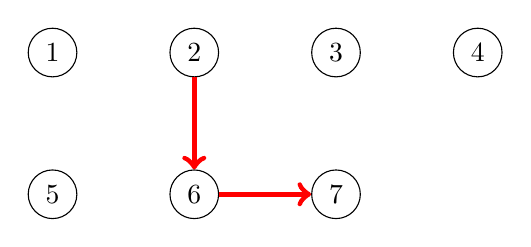
\begin{tikzpicture}[scale=0.9]
\node[draw, circle] (1) at (0,0) {1};
\node[draw, circle] (2) at (2,0) {2};
\node[draw, circle] (3) at (4,0) {3};
\node[draw, circle] (4) at (6,0) {4};
\node[draw, circle] (5) at (0,-2) {5};
\node[draw, circle] (6) at (2,-2) {6};
\node[draw, circle] (7) at (4,-2) {7};

\path[draw=red,thick,->,line width=2pt] (2) -- (6);
\path[draw=red,thick,->,line width=2pt] (6) -- (7);
\end{tikzpicture}
\end{center}

Uma cobertura geral mínima por caminhos pode ser encontrada
quase como uma cobertura mínima por caminhos disjuntos nos vértices.
Basta adicionar algumas arestas novas ao grafo de emparelhamento,
de forma que haja uma aresta $a \rightarrow b$
sempre que houver um caminho de $a$ para $b$
no grafo original (possivelmente através de várias arestas).

O grafo de emparelhamento para o grafo acima é o seguinte:
\begin{center}
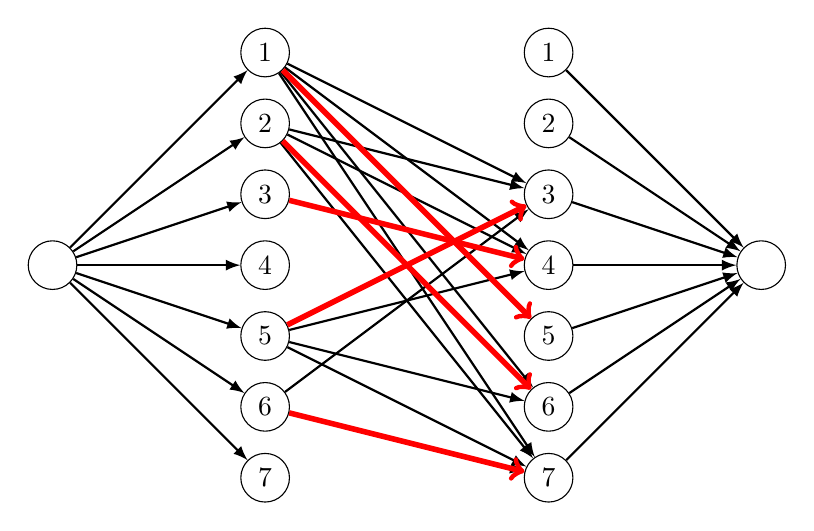
\begin{tikzpicture}[scale=0.9]
\node[draw, circle] (1a) at (0,6) {1};
\node[draw, circle] (2a) at (0,5) {2};
\node[draw, circle] (3a) at (0,4) {3};
\node[draw, circle] (4a) at (0,3) {4};
\node[draw, circle] (5a) at (0,2) {5};
\node[draw, circle] (6a) at (0,1) {6};
\node[draw, circle] (7a) at (0,0) {7};

\node[draw, circle] (1b) at (4,6) {1};
\node[draw, circle] (2b) at (4,5) {2};
\node[draw, circle] (3b) at (4,4) {3};
\node[draw, circle] (4b) at (4,3) {4};
\node[draw, circle] (5b) at (4,2) {5};
\node[draw, circle] (6b) at (4,1) {6};
\node[draw, circle] (7b) at (4,0) {7};

\node[draw, circle] (a) at (-3,3) {\phantom{0}};
\node[draw, circle] (b) at (7,3) {\phantom{0}};


%\path[draw,thick,->,>=latex] (1a) -- (5b);
\path[draw,thick,->,>=latex] (1a) -- (6b);
\path[draw,thick,->,>=latex] (1a) -- (7b);
\path[draw,thick,->,>=latex] (1a) -- (3b);
\path[draw,thick,->,>=latex] (1a) -- (4b);
\path[draw,thick,->,>=latex] (5a) -- (6b);
\path[draw,thick,->,>=latex] (5a) -- (7b);
%\path[draw,thick,->,>=latex] (5a) -- (3b);
\path[draw,thick,->,>=latex] (5a) -- (4b);
\path[draw,thick,->,>=latex] (6a) -- (7b);
%\path[draw,thick,->,>=latex] (6a) -- (7b);
\path[draw,thick,->,>=latex] (6a) -- (3b);
%\path[draw,thick,->,>=latex] (3a) -- (4b);
%\path[draw,thick,->,>=latex] (2a) -- (6b);
\path[draw,thick,->,>=latex] (2a) -- (7b);
\path[draw,thick,->,>=latex] (2a) -- (3b);
\path[draw,thick,->,>=latex] (2a) -- (4b);


\path[draw,thick,->,>=latex] (a) -- (1a);
\path[draw,thick,->,>=latex] (a) -- (2a);
\path[draw,thick,->,>=latex] (a) -- (3a);
\path[draw,thick,->,>=latex] (a) -- (4a);
\path[draw,thick,->,>=latex] (a) -- (5a);
\path[draw,thick,->,>=latex] (a) -- (6a);
\path[draw,thick,->,>=latex] (a) -- (7a);

\path[draw,thick,->,>=latex] (1b) -- (b);
\path[draw,thick,->,>=latex] (2b) -- (b);
\path[draw,thick,->,>=latex] (3b) -- (b);
\path[draw,thick,->,>=latex] (4b) -- (b);
\path[draw,thick,->,>=latex] (5b) -- (b);
\path[draw,thick,->,>=latex] (6b) -- (b);
\path[draw,thick,->,>=latex] (7b) -- (b);

\path[draw=red,thick,->,line width=2pt] (1a) -- (5b);
\path[draw=red,thick,->,line width=2pt] (5a) -- (3b);
\path[draw=red,thick,->,line width=2pt] (3a) -- (4b);
\path[draw=red,thick,->,line width=2pt] (2a) -- (6b);
\path[draw=red,thick,->,line width=2pt] (6a) -- (7b);


% \path[draw=red,thick,->,line width=2pt] (1a) -- (6b);
% \path[draw=red,thick,->,line width=2pt] (1a) -- (7b);
% \path[draw=red,thick,->,line width=2pt] (1a) -- (3b);
% \path[draw=red,thick,->,line width=2pt] (1a) -- (4b);
% \path[draw=red,thick,->,line width=2pt] (5a) -- (6b);
% \path[draw=red,thick,->,line width=2pt] (5a) -- (7b);
% \path[draw=red,thick,->,line width=2pt] (5a) -- (3b);
% \path[draw=red,thick,->,line width=2pt] (5a) -- (4b);
% \path[draw=red,thick,->,line width=2pt] (6a) -- (7b);
% \path[draw=red,thick,->,line width=2pt] (6a) -- (7b);
% \path[draw=red,thick,->,line width=2pt] (6a) -- (3b);
% \path[draw=red,thick,->,line width=2pt] (3a) -- (4b);
% \path[draw=red,thick,->,line width=2pt] (2a) -- (6b);
% \path[draw=red,thick,->,line width=2pt] (2a) -- (7b);
% \path[draw=red,thick,->,line width=2pt] (2a) -- (3b);
% \path[draw=red,thick,->,line width=2pt] (2a) -- (4b);

\end{tikzpicture}
\end{center}

\subsubsection{Teorema de Dilworth}

\index{Teorema de Dilworth}
\index{anticadeia}

Uma \key{anticadeia} é um conjunto de vértices de um grafo
tal que não existe um caminho
de qualquer vértice para outro vértice
usando as arestas do grafo.
O \key{Teorema de Dilworth} afirma que
em um grafo direcionado acíclico, o tamanho de
uma cobertura geral mínima por caminhos
é igual ao tamanho de uma anticadeia máxima.

Por exemplo, os vértices 3 e 7 formam uma anticadeia
no seguinte grafo:

\begin{center}
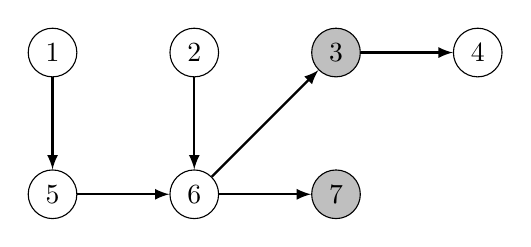
\begin{tikzpicture}[scale=0.9]
\node[draw, circle] (1) at (0,0) {1};
\node[draw, circle] (2) at (2,0) {2};
\node[draw, circle, fill=lightgray] (3) at (4,0) {3};
\node[draw, circle] (4) at (6,0) {4};
\node[draw, circle] (5) at (0,-2) {5};
\node[draw, circle] (6) at (2,-2) {6};
\node[draw, circle, fill=lightgray] (7) at (4,-2) {7};

\path[draw,thick,->,>=latex] (1) -- (5);
\path[draw,thick,->,>=latex] (2) -- (6);
\path[draw,thick,->,>=latex] (3) -- (4);
\path[draw,thick,->,>=latex] (5) -- (6);
\path[draw,thick,->,>=latex] (6) -- (3);
\path[draw,thick,->,>=latex] (6) -- (7);
\end{tikzpicture}
\end{center}

Esta é uma anticadeia máxima, pois não é possível
construir qualquer anticadeia que contenha três vértices.
Vimos anteriormente que o tamanho de uma cobertura geral mínima por caminhos
deste grafo consiste em dois caminhos.
